% the sample slide is created with 16:9 aspect ratio
\documentclass[aspectratio=169]{beamer}

\usepackage{mathpazo}
\usepackage{amssymb}
\usepackage{mathtools}
\usepackage[makeroom]{cancel}

\usetheme{saarland}

% the background and logo are in the images directory
\graphicspath{{figs/}}

% information for the title page
\author{Jason Yu}
\title{AP FRQ}
\subtitle{Worked problem 15}
\institute{University HS}
\date{\today}

\begin{document}
	\begin{frame}{Problem 15}
		A bullet of mass \(m\) and velocity \(v_0\) is fired toward a block of mass \(4m\). The block is initially at rest on a frictionless horizontal surface. The bullet penetrates the block and emerges with a velocity of \(\frac{v_0}{3}\)
		\begin{center}
			\only<1>{\tikzset{every picture/.style={line width=0.75pt}} %set default line width to 0.75pt        

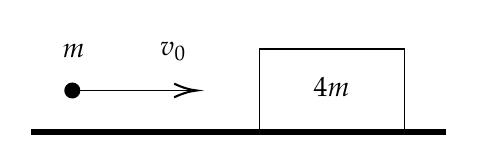
\begin{tikzpicture}[x=0.75pt,y=0.75pt,yscale=-1,xscale=1]
%uncomment if require: \path (0,284); %set diagram left start at 0, and has height of 284

%Straight Lines [id:da2354228935219831] 
\draw [line width=2.25]    (250,170) -- (450,170) ;
%Straight Lines [id:da4423200662416875] 
\draw    (270,150) -- (328,150) ;
\draw [shift={(330,150)}, rotate = 180] [color={rgb, 255:red, 0; green, 0; blue, 0 }  ][line width=0.75]    (10.93,-3.29) .. controls (6.95,-1.4) and (3.31,-0.3) .. (0,0) .. controls (3.31,0.3) and (6.95,1.4) .. (10.93,3.29)   ;
\draw [shift={(270,150)}, rotate = 0] [color={rgb, 255:red, 0; green, 0; blue, 0 }  ][fill={rgb, 255:red, 0; green, 0; blue, 0 }  ][line width=0.75]      (0, 0) circle [x radius= 3.35, y radius= 3.35]   ;
%Shape: Rectangle [id:dp013730634635779948] 
\draw   (360,130) -- (430,130) -- (430,170) -- (360,170) -- cycle ;
%Straight Lines [id:da8167829398208026] 
\draw [draw opacity=0][fill={rgb, 255:red, 255; green, 255; blue, 255 }  ,fill opacity=1 ]   (250,120) -- (450,120) ;

% Text Node
\draw (385,142.4) node [anchor=north west][inner sep=0.75pt]    {$4m$};
% Text Node
\draw (264,126.4) node [anchor=north west][inner sep=0.75pt]    {$m$};
% Text Node
\draw (311,125.4) node [anchor=north west][inner sep=0.75pt]    {$v_{0}$};

\end{tikzpicture}}
			\only<2>{\tikzset{every picture/.style={line width=0.75pt}} %set default line width to 0.75pt        

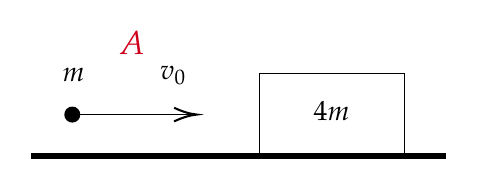
\begin{tikzpicture}[x=0.75pt,y=0.75pt,yscale=-1,xscale=1]
%uncomment if require: \path (0,284); %set diagram left start at 0, and has height of 284

%Straight Lines [id:da2354228935219831] 
\draw [line width=2.25]    (250,170) -- (450,170) ;
%Straight Lines [id:da4423200662416875] 
\draw    (270,150) -- (328,150) ;
\draw [shift={(330,150)}, rotate = 180] [color={rgb, 255:red, 0; green, 0; blue, 0 }  ][line width=0.75]    (10.93,-3.29) .. controls (6.95,-1.4) and (3.31,-0.3) .. (0,0) .. controls (3.31,0.3) and (6.95,1.4) .. (10.93,3.29)   ;
\draw [shift={(270,150)}, rotate = 0] [color={rgb, 255:red, 0; green, 0; blue, 0 }  ][fill={rgb, 255:red, 0; green, 0; blue, 0 }  ][line width=0.75]      (0, 0) circle [x radius= 3.35, y radius= 3.35]   ;
%Shape: Rectangle [id:dp013730634635779948] 
\draw   (360,130) -- (430,130) -- (430,170) -- (360,170) -- cycle ;
%Straight Lines [id:da8167829398208026] 
\draw [draw opacity=0][fill={rgb, 255:red, 255; green, 255; blue, 255 }  ,fill opacity=1 ]   (250,110) -- (450,110) ;

% Text Node
\draw (385,142.4) node [anchor=north west][inner sep=0.75pt]    {$4m$};
% Text Node
\draw (264,126.4) node [anchor=north west][inner sep=0.75pt]    {$m$};
% Text Node
\draw (311,125.4) node [anchor=north west][inner sep=0.75pt]    {$v_{0}$};
% Text Node
\draw (291,108.4) node [anchor=north west][inner sep=0.75pt]  [font=\large,color={rgb, 255:red, 208; green, 2; blue, 27 }  ,opacity=1 ]  {$A$};


\end{tikzpicture}}
			\only<3>{\tikzset{every picture/.style={line width=0.75pt}} %set default line width to 0.75pt        

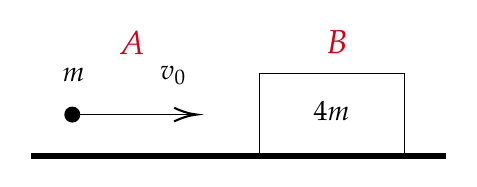
\begin{tikzpicture}[x=0.75pt,y=0.75pt,yscale=-1,xscale=1]
%uncomment if require: \path (0,284); %set diagram left start at 0, and has height of 284

%Straight Lines [id:da2354228935219831] 
\draw [line width=2.25]    (250,170) -- (450,170) ;
%Straight Lines [id:da4423200662416875] 
\draw    (270,150) -- (328,150) ;
\draw [shift={(330,150)}, rotate = 180] [color={rgb, 255:red, 0; green, 0; blue, 0 }  ][line width=0.75]    (10.93,-3.29) .. controls (6.95,-1.4) and (3.31,-0.3) .. (0,0) .. controls (3.31,0.3) and (6.95,1.4) .. (10.93,3.29)   ;
\draw [shift={(270,150)}, rotate = 0] [color={rgb, 255:red, 0; green, 0; blue, 0 }  ][fill={rgb, 255:red, 0; green, 0; blue, 0 }  ][line width=0.75]      (0, 0) circle [x radius= 3.35, y radius= 3.35]   ;
%Shape: Rectangle [id:dp013730634635779948] 
\draw   (360,130) -- (430,130) -- (430,170) -- (360,170) -- cycle ;
%Straight Lines [id:da8167829398208026] 
\draw [draw opacity=0][fill={rgb, 255:red, 255; green, 255; blue, 255 }  ,fill opacity=1 ]   (250,110) -- (450,110) ;

% Text Node
\draw (385,142.4) node [anchor=north west][inner sep=0.75pt]    {$4m$};
% Text Node
\draw (264,126.4) node [anchor=north west][inner sep=0.75pt]    {$m$};
% Text Node
\draw (311,125.4) node [anchor=north west][inner sep=0.75pt]    {$v_{0}$};
% Text Node
\draw (291,108.4) node [anchor=north west][inner sep=0.75pt]  [font=\large,color={rgb, 255:red, 208; green, 2; blue, 27 }  ,opacity=1 ]  {$A$};
% Text Node
\draw (391,108.4) node [anchor=north west][inner sep=0.75pt]  [font=\large,color={rgb, 255:red, 208; green, 2; blue, 27 }  ,opacity=1 ]  {$B$};

\end{tikzpicture}}
		\end{center}

		\begin{enumerate}[a)]
			\item Determine the final speed of the block.
			\item Determine the loss in kinetic energy of the bullet.
			\item Determine the gain in the kinetic energy of the block.
		\end{enumerate}
	\end{frame}

	\begin{frame}{Problem 15}
		\begin{enumerate}[a)]
			\item Determine the final speed of the block.
		\end{enumerate}
		\begin{center}
			\tikzset{every picture/.style={line width=0.75pt}} %set default line width to 0.75pt        

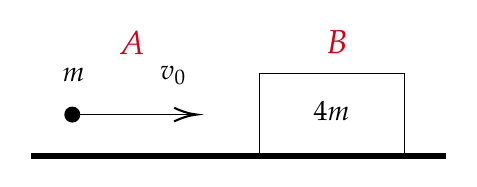
\begin{tikzpicture}[x=0.75pt,y=0.75pt,yscale=-1,xscale=1]
%uncomment if require: \path (0,284); %set diagram left start at 0, and has height of 284

%Straight Lines [id:da2354228935219831] 
\draw [line width=2.25]    (250,170) -- (450,170) ;
%Straight Lines [id:da4423200662416875] 
\draw    (270,150) -- (328,150) ;
\draw [shift={(330,150)}, rotate = 180] [color={rgb, 255:red, 0; green, 0; blue, 0 }  ][line width=0.75]    (10.93,-3.29) .. controls (6.95,-1.4) and (3.31,-0.3) .. (0,0) .. controls (3.31,0.3) and (6.95,1.4) .. (10.93,3.29)   ;
\draw [shift={(270,150)}, rotate = 0] [color={rgb, 255:red, 0; green, 0; blue, 0 }  ][fill={rgb, 255:red, 0; green, 0; blue, 0 }  ][line width=0.75]      (0, 0) circle [x radius= 3.35, y radius= 3.35]   ;
%Shape: Rectangle [id:dp013730634635779948] 
\draw   (360,130) -- (430,130) -- (430,170) -- (360,170) -- cycle ;
%Straight Lines [id:da8167829398208026] 
\draw [draw opacity=0][fill={rgb, 255:red, 255; green, 255; blue, 255 }  ,fill opacity=1 ]   (250,110) -- (450,110) ;

% Text Node
\draw (385,142.4) node [anchor=north west][inner sep=0.75pt]    {$4m$};
% Text Node
\draw (264,126.4) node [anchor=north west][inner sep=0.75pt]    {$m$};
% Text Node
\draw (311,125.4) node [anchor=north west][inner sep=0.75pt]    {$v_{0}$};
% Text Node
\draw (291,108.4) node [anchor=north west][inner sep=0.75pt]  [font=\large,color={rgb, 255:red, 208; green, 2; blue, 27 }  ,opacity=1 ]  {$A$};
% Text Node
\draw (391,108.4) node [anchor=north west][inner sep=0.75pt]  [font=\large,color={rgb, 255:red, 208; green, 2; blue, 27 }  ,opacity=1 ]  {$B$};

\end{tikzpicture}
		\end{center}
		\begin{align*}
			\only<2>{m_A v_A + m_B v_B &= m_A v_A' + m_B v_B' \tag{Conservation of Momentum} \\}
			\onslide<3->{m_A v_A + \cancel{m_B v_B} &= m_A v_A' + m_B v_B' \\}
			\onslide<4->{m v_0 &= m(\frac{v_0}{3}) + (4m)v_B' \\}
			\only<5>{mv_0 - \frac{mv_0}{3} &= 4mv_B' \\}
			\onslide<6->{\cancel{m}v_0 - \frac{\cancel{m}v_0}{3} &= 4\cancel{m}v_B' \\}
			\onslide<7->{v_B' &= \frac{1}{4}(v_0 - \frac{v_0}{3}) \\}
			\onslide<8->{\Aboxed{v_B' &= \frac{v_0}{6}}}
		\end{align*}
	\end{frame}

	\begin{frame}{Problem 15}
		\begin{enumerate}[a)]
			\setcounter{enumi}{1}
			\item Determine the loss in kinetic energy of the bullet.
		\end{enumerate}
		\begin{equation*}
			\onslide<2->{K = \frac{1}{2}mv^2}
		\end{equation*}
		\vskip -2em
		\begin{columns}
			\column{0.5\textwidth}
			\begin{align*}
				\onslide<3->{\Aboxed{K_A &= \frac{1}{2} mv_0^2} \\}
				\onslide<4->{K_A' &= \frac{1}{2}mv_A'^2 \\}
				\onslide<5->{ &= \frac{1}{2}m\left(\frac{v_0}{3}\right)^2 \\}
				\onslide<6->{\Aboxed{K_A' &= \frac{mv_0^2}{18}}}
			\end{align*}

			\column{0.5\textwidth}
			\begin{center}
				\tikzset{every picture/.style={line width=0.75pt}} %set default line width to 0.75pt        

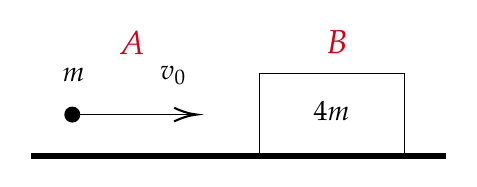
\begin{tikzpicture}[x=0.75pt,y=0.75pt,yscale=-1,xscale=1]
%uncomment if require: \path (0,284); %set diagram left start at 0, and has height of 284

%Straight Lines [id:da2354228935219831] 
\draw [line width=2.25]    (250,170) -- (450,170) ;
%Straight Lines [id:da4423200662416875] 
\draw    (270,150) -- (328,150) ;
\draw [shift={(330,150)}, rotate = 180] [color={rgb, 255:red, 0; green, 0; blue, 0 }  ][line width=0.75]    (10.93,-3.29) .. controls (6.95,-1.4) and (3.31,-0.3) .. (0,0) .. controls (3.31,0.3) and (6.95,1.4) .. (10.93,3.29)   ;
\draw [shift={(270,150)}, rotate = 0] [color={rgb, 255:red, 0; green, 0; blue, 0 }  ][fill={rgb, 255:red, 0; green, 0; blue, 0 }  ][line width=0.75]      (0, 0) circle [x radius= 3.35, y radius= 3.35]   ;
%Shape: Rectangle [id:dp013730634635779948] 
\draw   (360,130) -- (430,130) -- (430,170) -- (360,170) -- cycle ;
%Straight Lines [id:da8167829398208026] 
\draw [draw opacity=0][fill={rgb, 255:red, 255; green, 255; blue, 255 }  ,fill opacity=1 ]   (250,110) -- (450,110) ;

% Text Node
\draw (385,142.4) node [anchor=north west][inner sep=0.75pt]    {$4m$};
% Text Node
\draw (264,126.4) node [anchor=north west][inner sep=0.75pt]    {$m$};
% Text Node
\draw (311,125.4) node [anchor=north west][inner sep=0.75pt]    {$v_{0}$};
% Text Node
\draw (291,108.4) node [anchor=north west][inner sep=0.75pt]  [font=\large,color={rgb, 255:red, 208; green, 2; blue, 27 }  ,opacity=1 ]  {$A$};
% Text Node
\draw (391,108.4) node [anchor=north west][inner sep=0.75pt]  [font=\large,color={rgb, 255:red, 208; green, 2; blue, 27 }  ,opacity=1 ]  {$B$};

\end{tikzpicture}
			\end{center}
			\begin{align*}
				\onslide<7->{\Delta K_A &= K_A' - K_A \\}
				\onslide<8->{&= \frac{1}{18}mv_0^2 - \frac{1}{2}mv_0^2 \\}
				\onslide<9->{\Aboxed{\Delta K_A &= -\frac{4}{9}mv_0^2}}
			\end{align*}
		\end{columns}
	\end{frame}

	\begin{frame}{Problem 15}
		\begin{enumerate}[a)]
			\setcounter{enumi}{2}
			\item Determine the gain in the kinetic energy of the block.
		\end{enumerate}
		\begin{center}
			\tikzset{every picture/.style={line width=0.75pt}} %set default line width to 0.75pt        

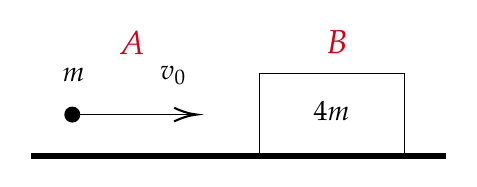
\begin{tikzpicture}[x=0.75pt,y=0.75pt,yscale=-1,xscale=1]
%uncomment if require: \path (0,284); %set diagram left start at 0, and has height of 284

%Straight Lines [id:da2354228935219831] 
\draw [line width=2.25]    (250,170) -- (450,170) ;
%Straight Lines [id:da4423200662416875] 
\draw    (270,150) -- (328,150) ;
\draw [shift={(330,150)}, rotate = 180] [color={rgb, 255:red, 0; green, 0; blue, 0 }  ][line width=0.75]    (10.93,-3.29) .. controls (6.95,-1.4) and (3.31,-0.3) .. (0,0) .. controls (3.31,0.3) and (6.95,1.4) .. (10.93,3.29)   ;
\draw [shift={(270,150)}, rotate = 0] [color={rgb, 255:red, 0; green, 0; blue, 0 }  ][fill={rgb, 255:red, 0; green, 0; blue, 0 }  ][line width=0.75]      (0, 0) circle [x radius= 3.35, y radius= 3.35]   ;
%Shape: Rectangle [id:dp013730634635779948] 
\draw   (360,130) -- (430,130) -- (430,170) -- (360,170) -- cycle ;
%Straight Lines [id:da8167829398208026] 
\draw [draw opacity=0][fill={rgb, 255:red, 255; green, 255; blue, 255 }  ,fill opacity=1 ]   (250,110) -- (450,110) ;

% Text Node
\draw (385,142.4) node [anchor=north west][inner sep=0.75pt]    {$4m$};
% Text Node
\draw (264,126.4) node [anchor=north west][inner sep=0.75pt]    {$m$};
% Text Node
\draw (311,125.4) node [anchor=north west][inner sep=0.75pt]    {$v_{0}$};
% Text Node
\draw (291,108.4) node [anchor=north west][inner sep=0.75pt]  [font=\large,color={rgb, 255:red, 208; green, 2; blue, 27 }  ,opacity=1 ]  {$A$};
% Text Node
\draw (391,108.4) node [anchor=north west][inner sep=0.75pt]  [font=\large,color={rgb, 255:red, 208; green, 2; blue, 27 }  ,opacity=1 ]  {$B$};

\end{tikzpicture}
		\end{center}
		\begin{align*}
			\onslide<2->{K_B &= 0 \\}
			\onslide<3->{K_B' &= \frac{1}{2}m_B v_B'^2 \\}
			\onslide<4->{&= \frac{1}{2}(4m)\left(\frac{v_0}{6}\right)^2 = \frac{1}{18}mv^2_0 \\}
			\onslide<5->{\Aboxed{\Delta K_B &= K_B' - K_B = \frac{1}{18}mv^2_0}}
		\end{align*}
	\end{frame}
\end{document}
